\documentclass[11pt]{article}

\usepackage[T1]{fontenc}
\usepackage{amsmath,amssymb}
\usepackage{booktabs}
\usepackage{geometry}
\usepackage{graphicx}
\usepackage{hyperref}
\usepackage{microtype}
\usepackage{xcolor}

\geometry{margin=1in}
\graphicspath{{../}{calculations/piab1d/}}
\hypersetup{colorlinks=true,linkcolor=blue!55!black,urlcolor=blue!55!black}

\newcommand{\fro}{\mathrm{F}}
\newcommand{\RR}{\mathbb{R}}
\newcommand{\code}[1]{\texttt{#1}}

\title{PIAB1D Spectral Reduction\\
\large Finite Dirichlet calibration and interpretation report}
\author{Project Koios}
\date{\today}

\begin{document}
\maketitle

\begin{center}
\fbox{\begin{minipage}{0.92\linewidth}
\textbf{Status.} This is a technical report for
\code{calculations/piab1d}.  The retained JSON and graphics are calculated
illustrative numerical evidence.  They are not semiconductor evidence, material-model
validation, uncertainty quantification, or a claim that a reduced residual has a
unique physical interpretation.  Exact Lean results are a separate evidence layer and
do not certify the binary64 arrays retained here.
\end{minipage}}
\end{center}

\begin{abstract}
The one-dimensional particle in a box is used as an exact calibration problem for
spectral reduction.  A centered finite-difference Dirichlet Hamiltonian is fixed first;
its lowest eigenvectors then define an invariant retained subspace.  In exact
arithmetic the reduced matrix is diagonal, trial-space leakage vanishes, and sampled
continuum sine modes span the same subspace as the discrete eigenvectors.  The
remaining spectral discrepancy is therefore finite-difference dispersion rather than
failure of the reduction map.  Retained calculations verify the closed-form finite
spectrum, fixed-mode second-order behavior, nonuniform high-index dispersion,
projector and embedding identities, and the dependence of residual interpretation on
compression, reference operator, norm, and admissible model class.  PIAB1D thereby
provides the exact finite calibration case for later QHO1D spatial-truncation
diagnostics.
\end{abstract}

\section{Question and scope}

The central question is not how to solve the particle-in-a-box spectrum.  Both the
continuum and centered finite-difference spectra are known.  The question is what is
preserved, discarded, or reinterpreted when a finite Hamiltonian is spectrally reduced.

The order of construction matters:
\begin{enumerate}
\item declare the continuum operator and boundary domain;
\item construct one finite Dirichlet realization on a declared grid;
\item select an invariant low-energy subspace of that finite matrix;
\item distinguish full-space embedding from retained coordinates; and
\item only then form differences or apply norms.
\end{enumerate}

This is a spectral-reduction study, not a study of an isolated finite barrier, an
asymptotic scattering problem, or a periodic Bloch supercell.  The homogeneous
Dirichlet boundary is part of the box operator realization.

\section{Continuum and finite Dirichlet spectra}

For a particle of mass $m$ on $(0,L)$, the continuum reference is
\begin{equation}
 \widehat H_{\mathrm{box}}
 =-\frac{\hbar^2}{2m}\frac{d^2}{dx^2},
 \qquad
 \mathcal D(\widehat H_{\mathrm{box}})=H^2(0,L)\cap H_0^1(0,L).
\end{equation}
Its eigenpairs are
\begin{equation}
 \psi_n(x)=\sqrt{\frac{2}{L}}\sin\!\left(\frac{n\pi x}{L}\right),
 \qquad
 E_n=\frac{\hbar^2\pi^2n^2}{2mL^2},
 \qquad n\geq 1.
\end{equation}
The interior physical potential is zero.  Confinement is encoded by the operator
domain rather than by a finite-valued multiplication potential; see
Ref.~\cite{teschl2014} for the operator-theoretic setting.

For $N$ interior points and $h=L/(N+1)$, the finite state space is
$\mathcal V_h\cong\RR^N$.  The centered Dirichlet matrix is
\begin{equation}
 H_h=\frac{\hbar^2}{2mh^2}
 \begin{bmatrix}
 2&-1&&0\\
 -1&2&\ddots&\\
 &\ddots&\ddots&-1\\
 0&&-1&2
 \end{bmatrix}.
 \label{eq:finite-hamiltonian}
\end{equation}
This is the standard centered second-order finite-difference realization
\cite{strikwerda2004}. Its normalized eigenvectors are discrete sine modes, and its
eigenvalues are
\begin{equation}
 \lambda_{n,h}
 =\frac{2\hbar^2}{mh^2}
 \sin^2\!\left(\frac{n\pi}{2(N+1)}\right),
 \qquad n=1,\ldots,N.
 \label{eq:discrete-spectrum}
\end{equation}
The finite and continuum spectra are separate exact formulas.  Agreement of a
numerical eigensolver with Equation~\eqref{eq:discrete-spectrum} does not establish
agreement with $E_n$.

\section{Exact spectral reduction of the finite matrix}

Let $U_M\in\RR^{N\times M}$ contain the lowest $M$ normalized eigenvectors of $H_h$.
Define
\begin{equation}
 P_M=U_MU_M^{\mathsf T},
 \qquad
 Q_M=I_N-P_M,
 \qquad
 H_{\mathrm{red}}=U_M^{\mathsf T}H_hU_M.
\end{equation}
By the finite-dimensional spectral theorem and orthogonal compression
\cite{hornJohnson2013,golubVanLoan2013}, because
$\operatorname{range}(U_M)$ is a spectral subspace,
\begin{equation}
 H_hU_M=U_M\Lambda_{M,h},
 \qquad
 H_{\mathrm{red}}=\Lambda_{M,h},
 \qquad
 Q_MH_hU_M=0
 \label{eq:exact-reduction}
\end{equation}
in exact arithmetic.  Thus the reduction has no finite-matrix trial-space leakage.

The embedded retained operator
\begin{equation}
 H_h^{(P_M)}=P_MH_hP_M\in\RR^{N\times N}
\end{equation}
and the retained-coordinate matrix
$H_{\mathrm{red}}\in\RR^{M\times M}$ describe the same restriction in different
representations.  They cannot be subtracted without an explicit embedding or
coordinate map.

The analytically sampled sine columns and the discrete spectral columns span the same
subspace, up to signs.  The basis-independent comparison is therefore
\begin{equation}
 P_{\mathrm{sine}}-P_M,
\end{equation}
not a raw difference between sign-ambiguous eigenvector columns.  This makes PIAB1D an
exact calibration for projector, leakage, reduction, and retained-coordinate
diagnostics.

\section{Discrete reduction versus continuum approximation}

Two analytical-reference choices separate the two questions.  With
\begin{equation}
 D_h=\operatorname{diag}(\lambda_{1,h},\ldots,\lambda_{M,h}),
\end{equation}
Equation~\eqref{eq:exact-reduction} gives
\begin{equation}
 H_hU_M-U_MD_h=0.
\end{equation}
With the continuum reference
\begin{equation}
 D=\operatorname{diag}(E_1,\ldots,E_M),
\end{equation}
one instead has
\begin{equation}
 H_hU_M-U_MD=U_M(D_h-D).
 \label{eq:dispersion-residual}
\end{equation}
There is still no leakage from the retained finite eigenspace.  The residual in
Equation~\eqref{eq:dispersion-residual} is the discrete-to-continuum dispersion error.
It must not be labeled reduction error.

\section{Retained core calculation}

The core calculation uses the dimensionless convention $L=m=\hbar=1$, with $N=8$
interior points and $M=3$ retained modes.  Independent verification reports:
\begin{table}[ht]
\centering
\begin{tabular}{@{}lr@{}}
\toprule
Diagnostic & Calculated value \\
\midrule
Maximum absolute error against the closed-form discrete spectrum
 & $8.53\times10^{-14}$ \\
Spectral reconstruction Frobenius error & $3.04\times10^{-13}$ \\
Projector idempotency Frobenius error & $8.48\times10^{-16}$ \\
Retained-coordinate Frobenius error & $2.46\times10^{-14}$ \\
Retained embedding Frobenius error & $1.02\times10^{-14}$ \\
\bottomrule
\end{tabular}
\caption{Binary64 checks for the retained spectral reduction.}
\label{tab:core-diagnostics}
\end{table}

These values diagnose implementation agreement with exact finite formulas.  They are
not interval enclosures and do not assign a physical meaning to a later matrix
subtraction.

\begin{figure}[ht]
\centering
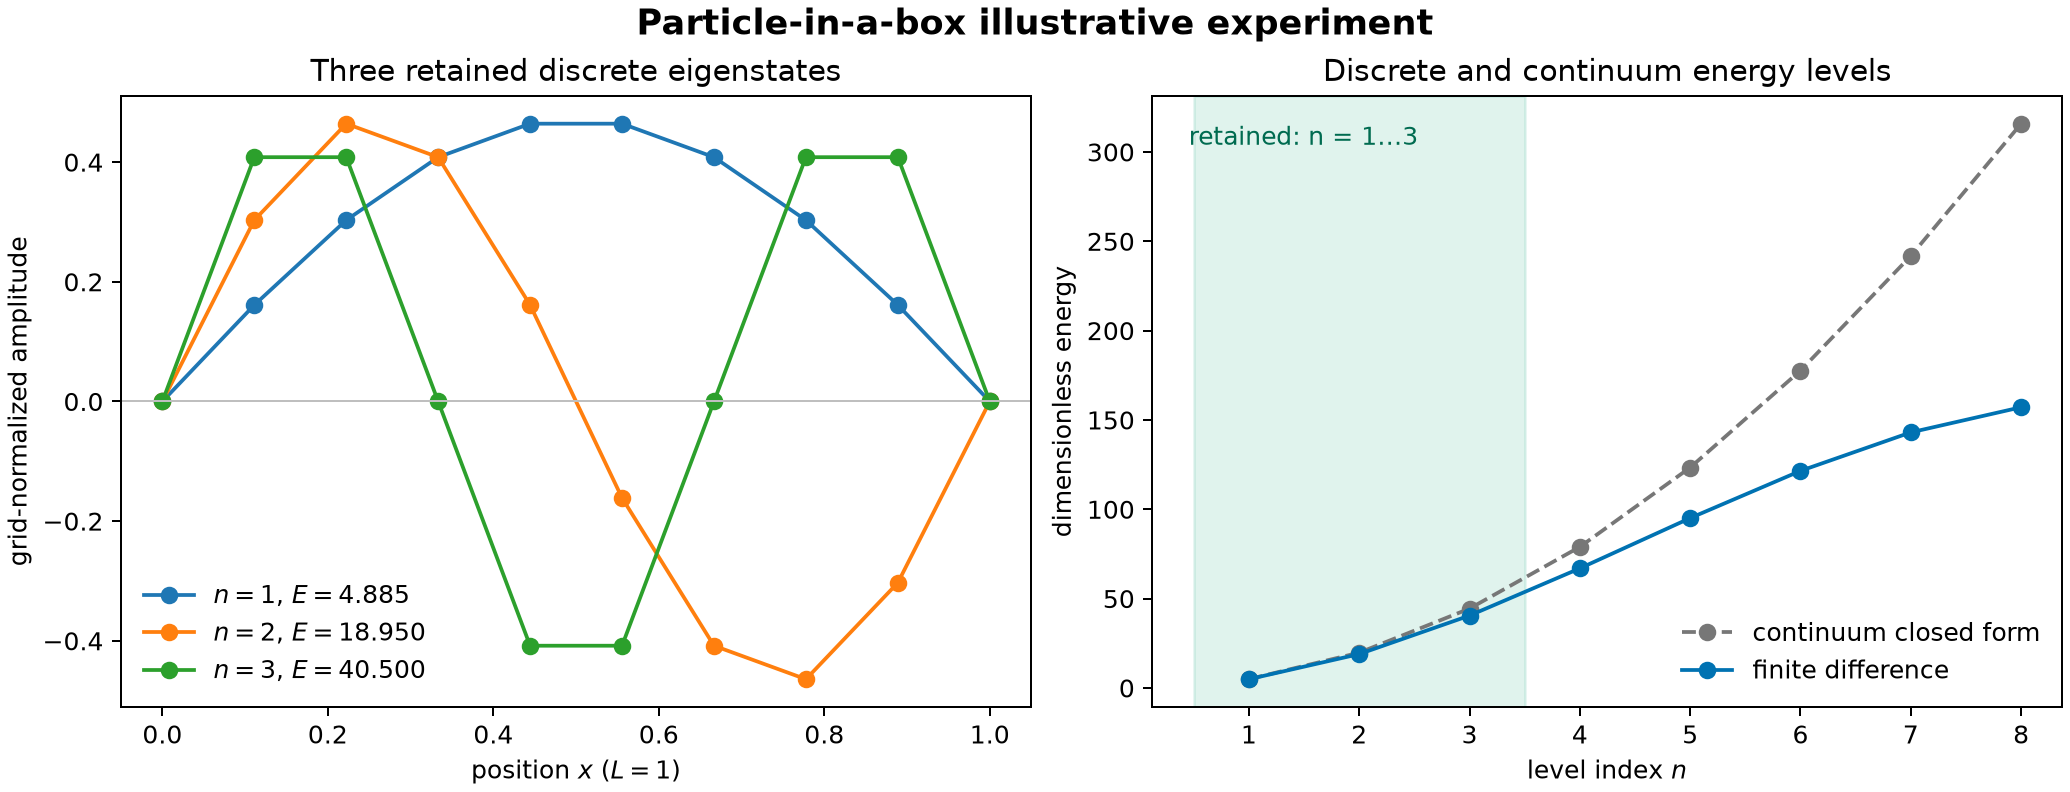
\includegraphics[width=\linewidth]{spectrum-and-states.png}
\caption{The lowest retained discrete states and the finite and continuum spectra.
Nodal agreement and accurate discrete eigenpairs are distinct from continuum spectral
accuracy.}
\label{fig:spectrum}
\end{figure}

\section{Fixed-mode convergence and high-index dispersion}

The grid refinement sequence is
\begin{equation}
 N=8,16,32,64,128,256.
\end{equation}
At $N=256$, the relative energy errors for fixed modes $n=1,2,3$ are
\begin{equation}
 1.2452\times10^{-5},\qquad
 4.9809\times10^{-5},\qquad
 1.1207\times10^{-4}.
\end{equation}
Their final observed refinement orders are $1.99998$, $1.99991$, and $1.99981$.
This is bounded numerical evidence for the expected second-order behavior of fixed,
resolved modes.

\begin{figure}[ht]
\centering
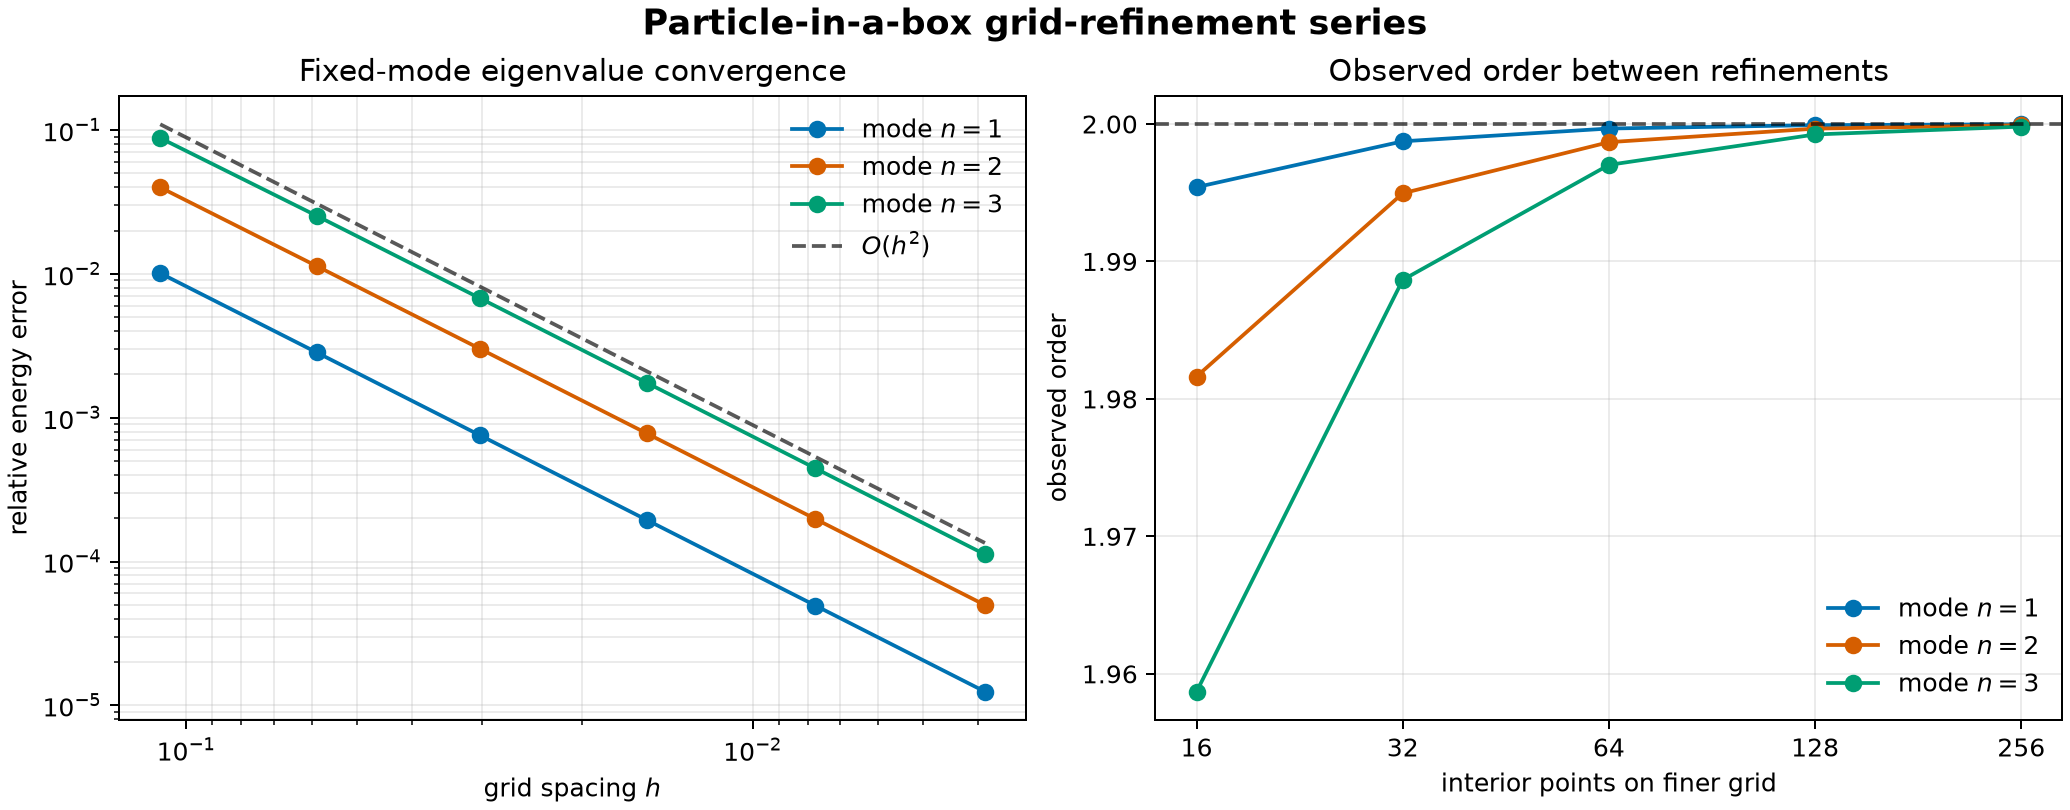
\includegraphics[width=0.92\linewidth]{convergence-series.png}
\caption{Fixed low-mode relative energy errors across the retained grid sequence.}
\label{fig:fixed-mode-convergence}
\end{figure}

Fixed-index convergence is not uniform convergence of the growing spectrum.  If the
fractional mode index $q=n/(N+1)$ remains approximately fixed, the finite-difference
dispersion remains substantial.  At $N=256$, representative relative errors are about
$0.0500$ near $q=0.25$, $0.188$ near $q=0.50$, $0.386$ near $q=0.75$, and $0.592$
near $q=1$.  The corresponding scaled algebraic eigenpair residuals remain at
binary64 roundoff.  The eigensolver can therefore be accurate while the continuum
approximation is poor.

\begin{figure}[ht]
\centering
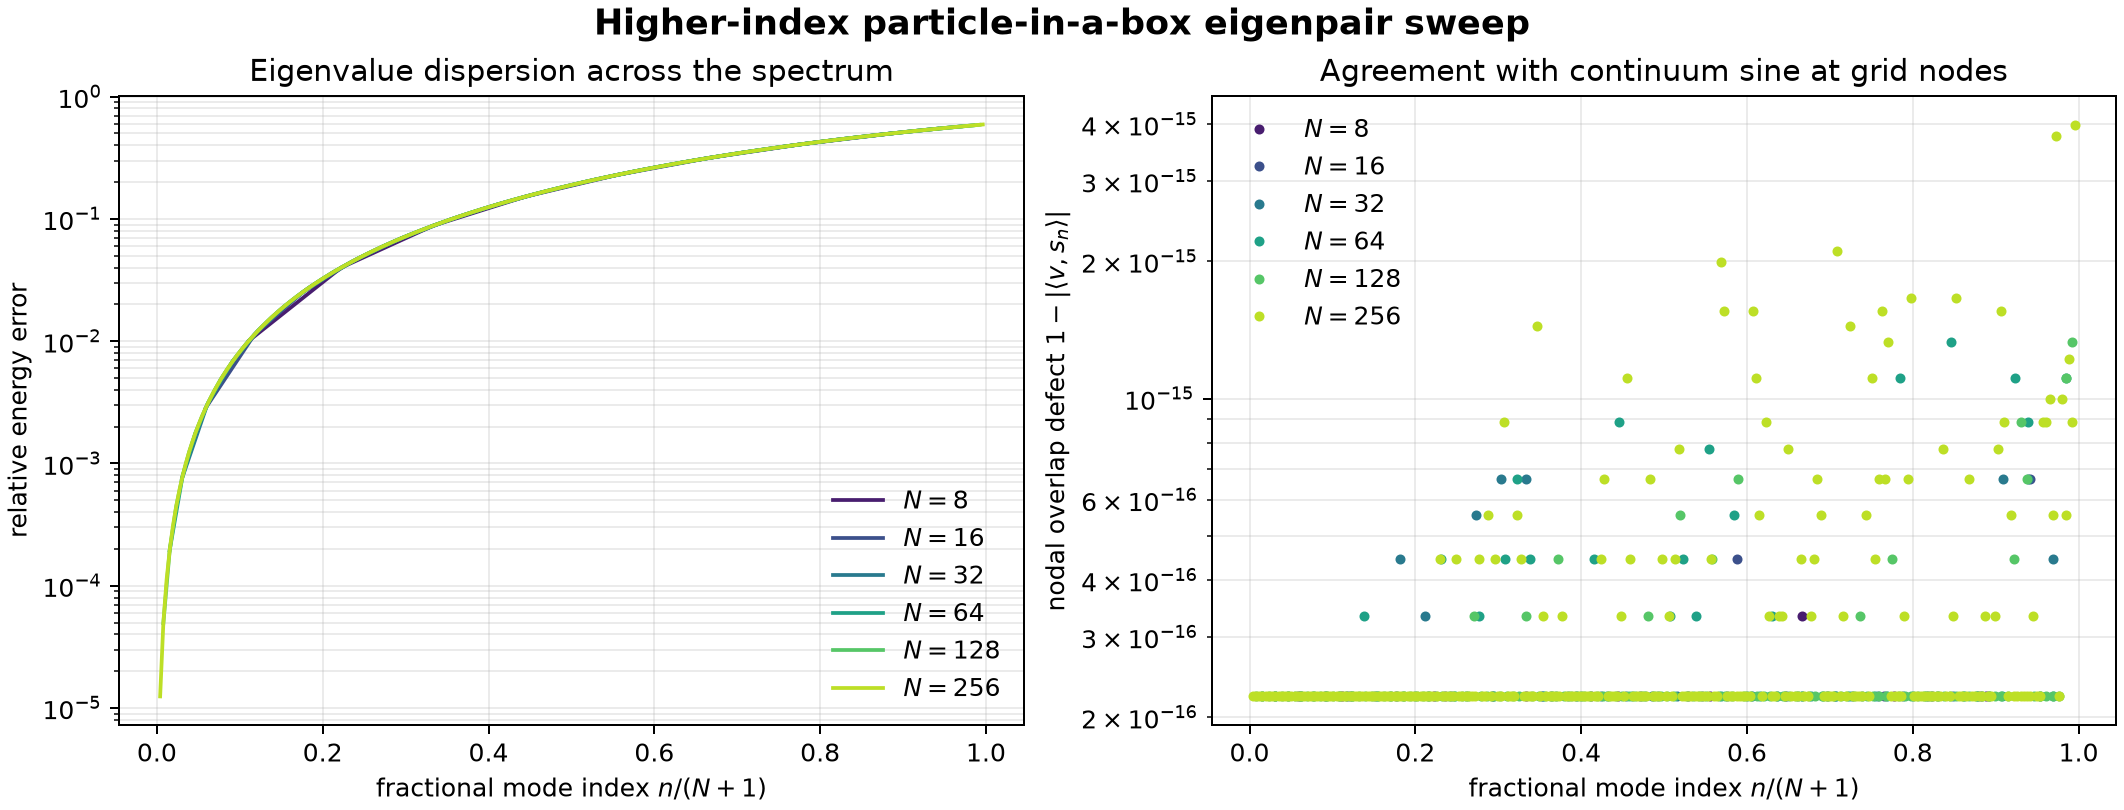
\includegraphics[width=\linewidth]{higher-eigenpair-sweep.png}
\caption{Full-spectrum finite-difference dispersion and nodal eigenvector checks.}
\label{fig:full-spectrum}
\end{figure}

\section{Three different residual constructions}

For this model the finite Hamiltonian equals the finite Dirichlet kinetic operator:
\begin{equation}
 H_h=T_{\mathrm D,h}.
\end{equation}
Consistent compression therefore gives
\begin{equation}
 P_MH_hP_M-P_MT_{\mathrm D,h}P_M=0.
 \label{eq:consistent-compression}
\end{equation}
This zero is the consistently reduced physical potential for the declared box model.

If only the Hamiltonian is compressed, then
\begin{equation}
 P_MH_hP_M-T_{\mathrm D,h}
 =-Q_MT_{\mathrm D,h}Q_M.
 \label{eq:unmatched-compression}
\end{equation}
For $N=8$ and $M=3$, its calculated Frobenius norm is $270.977$, with
$8.75\times10^{-14}$ error against the discarded-sector oracle.  The nonzero matrix is
a consequence of unmatched reduction, not the physical box potential.

A third difference compares two finite boundary realizations:
\begin{equation}
 B_h=H_{\mathrm D,h}-H_{\mathrm{cyclic},h}.
 \label{eq:boundary-difference}
\end{equation}
At $N=8$, its Frobenius norm is $57.276$.  The matrix contains the two corner
couplings by which the cyclic closure differs from the Dirichlet closure.  It is a
declared finite-space reference difference, not a representation-independent
continuum potential.

\begin{figure}[ht]
\centering
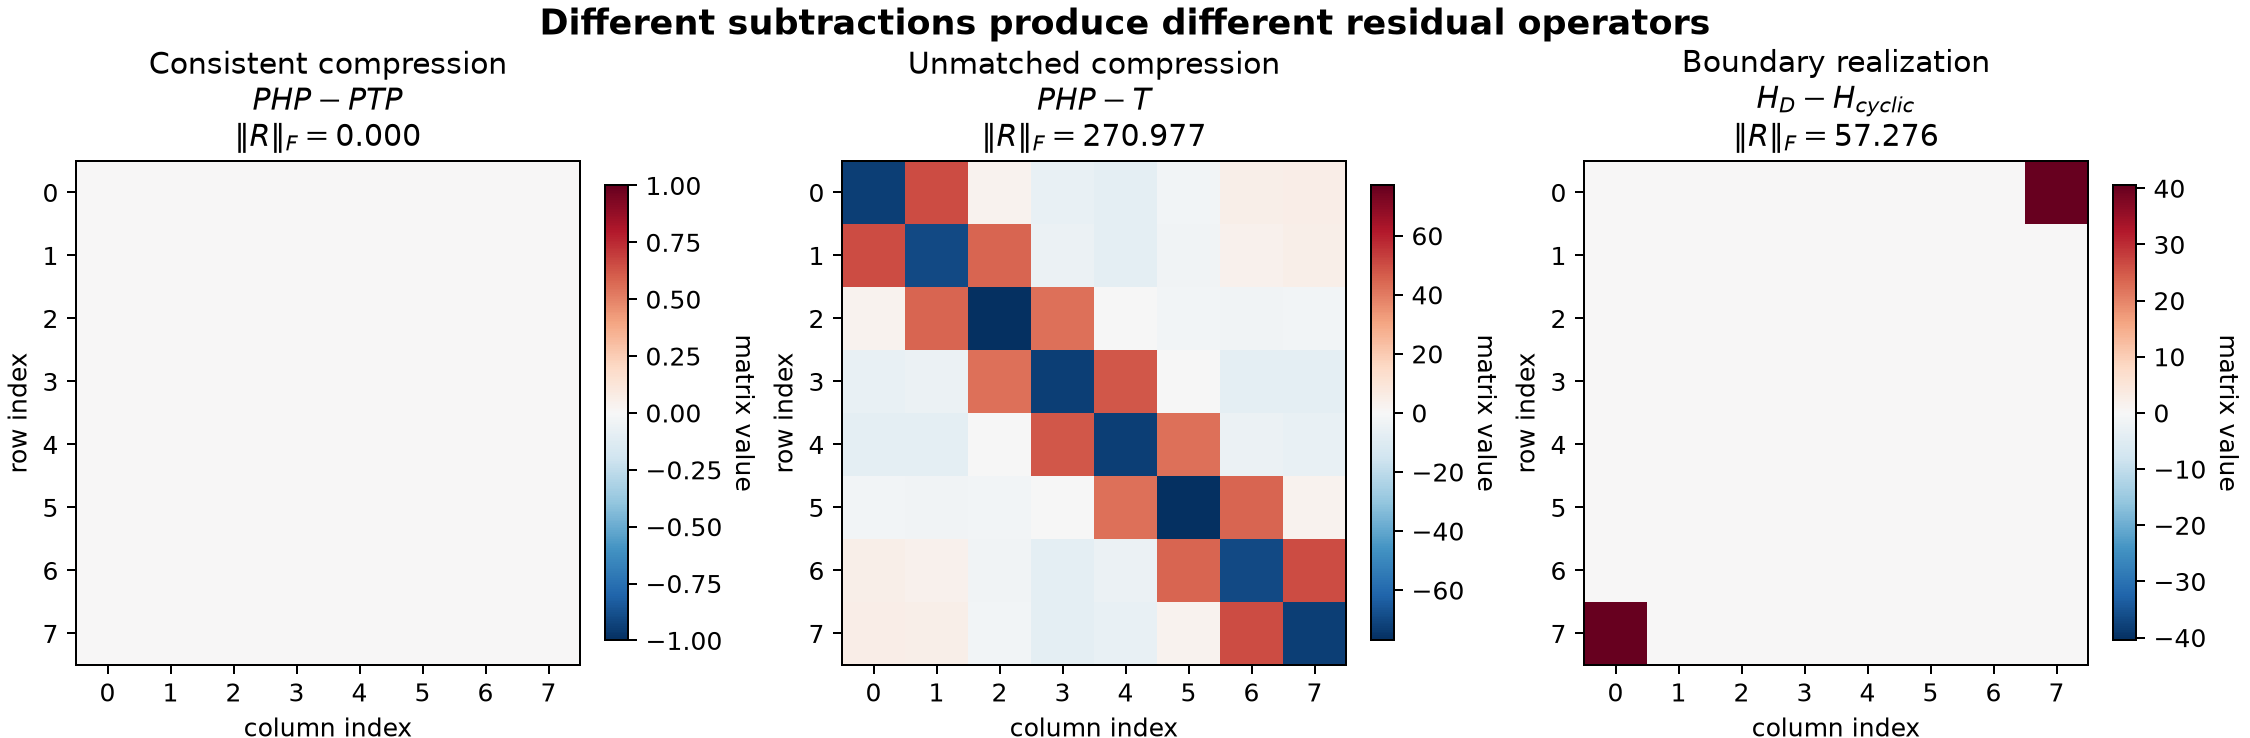
\includegraphics[width=\linewidth]{residual-matrices.png}
\caption{Consistent compression, unmatched compression, and boundary-realization
difference.  Similar subtraction syntax does not imply common semantics.}
\label{fig:residuals}
\end{figure}

\section{Norms are observations of an aligned residual}

A matrix norm becomes meaningful only after dimensions, coordinates, ordering, units,
energy reference, embedding, and subtraction sign have been declared.  The reduction
itself produces a matrix; a later experiment selects the observation norm.

The boundary difference in Equation~\eqref{eq:boundary-difference} illustrates the
point.  As $N$ grows, its Hamiltonian-normalized Frobenius norm decreases, its
normalized spectral norm approaches approximately $0.25$, and its normalized
maximum-entry norm remains $0.5$.  These statements are compatible because the norms
measure aggregate magnitude, worst-case Euclidean action, and basis-local entry size,
respectively.

Raw norms are not interpreted as convergence metrics across changing dimensions: the
state space grows and the kinetic scale varies as $h^{-2}$.

\section{Reduction does not identify a kinetic--potential split}

For admissible kinetic and potential classes $\mathcal K$ and $\mathcal V$, define the
decomposition fiber
\begin{equation}
 \mathcal D_H(\mathcal K,\mathcal V)
 =\{(T,V):T\in\mathcal K,\ V\in\mathcal V,\ H=T+V\}.
\end{equation}
Global additive identifiability requires
\begin{equation}
 (\mathcal K-\mathcal K)\cap(\mathcal V-\mathcal V)=\{0\}.
\end{equation}

The retained $M=3$ calculation records both
\begin{equation}
 H_{\mathrm{red}}=T_{\mathrm D,red}+0
\end{equation}
and, for a declared real-symmetric shift $K$,
\begin{equation}
 H_{\mathrm{red}}=(T_{\mathrm D,red}-K)+K.
\end{equation}
The second equality is algebraically exact up to binary64 replay error, but it gives
$K$ no physical status.  Fitting the illustrative shift to scalar, diagonal,
tridiagonal, and unrestricted real-symmetric classes leaves Frobenius residuals
$1.9967$, $1.8561$, $0.5657$, and $0$, respectively.  A unique optimum in one chosen
class is model-relative fitting, not physical identification.

\section{Formal crosswalk and evidence boundary}

The companion \code{projectkoios-formal} PIAB1D development uses Lean~4 and mathlib
\cite{demouraUllrich2021,mathlib2020} to prove exact statements about:
\begin{itemize}
\item centered Dirichlet recurrences and matrix realization;
\item reciprocal-character construction of sine modes;
\item mode reality and normalization;
\item exact finite \code{Matrix.mulVec} eigenpairs;
\item spacing scaling and cosine-form eigenvalues;
\item orthogonal compression identities; and
\item additive decomposition nonuniqueness and finite model-class fitting.
\end{itemize}
The spectral tranche begins at local formal commit
\begin{center}
\small\code{e5af20c0f7876300723dc66ac7eceae788fc727c}.
\end{center}
Later twisted-boundary and finite-barrier commits are separate from the retained
spectral-reduction calculation.

The exact proofs do not certify the retained JSON bytes, NumPy or SciPy execution,
binary64 eigensolvers, or the plotted figures.  The numerical verifiers independently
reconstruct the declared finite formulas, but they do not prove uniform continuum
convergence or material applicability.

\section{Relation to QHO1D}

PIAB1D is the exact finite calibration case.  The analytical sine trial subspace and
the finite spectral subspace coincide, so projector mismatch and leakage vanish in
exact arithmetic.  QHO1D changes the question: sampled real-line Hermite states are
placed on a finite Dirichlet box and generally do not span an invariant subspace of
the finite spatial Hamiltonian.

The common diagnostic vocabulary is therefore:
\begin{align}
 \text{isometry defect} &:
   J^{\mathsf T}J-I,\\
 \text{trial leakage} &:
   (I-JJ^{\mathsf T})H_hJ,\\
 \text{analytical residual} &:
   H_hJ-JD,\\
 \text{subspace difference} &:
   JJ^{\mathsf T}-UU^{\mathsf T},\\
 \text{retained operator} &:
   J^{\mathsf T}H_hJ.
\end{align}
PIAB1D supplies their exact spectral baseline.  QHO1D uses the same leaves to expose
finite-box, boundary-row, interior-stencil, Gram, projection, and floating-point
channels.

\section{Reproduction and conclusions}

From the repository's \code{python/} directory, the retained verification commands
include
\begin{verbatim}
uv run python ../calculations/piab1d/verify_result.py \
  ../calculations/piab1d/result.json
uv run python ../calculations/piab1d/verify_convergence.py \
  ../calculations/piab1d/convergence-result.json
uv run python ../calculations/piab1d/verify_eigenpair_sweep.py \
  ../calculations/piab1d/eigenpair-sweep-result.json
uv run python ../calculations/piab1d/verify_norm_sweep.py \
  ../calculations/piab1d/norm-sweep-result.json
uv run python ../calculations/piab1d/verify_identifiability.py \
  ../calculations/piab1d/identifiability-result.json
\end{verbatim}
The exact artifact inventory and digests are recorded in \code{../SHA256SUMS}.

PIAB1D establishes an exact finite spectral-reduction baseline: the selected subspace
is invariant, the reduced matrix is known, and leakage vanishes.  The substantive
approximation is discrete-to-continuum dispersion, which is second order for each fixed
resolved mode but not uniform over the growing spectrum.  The residual studies further
show that compression, reference selection, norm choice, and admissible model class
must remain explicit before a matrix difference receives physical meaning.

\bibliographystyle{plain}
\bibliography{references}

\end{document}
